\documentclass[a4paper,11pt,abstracton,twoside,titlepage,openany,nochapterprefix,noappendixprefix,liststotoc,bibtotoc,normalheadings,pointlessnumbers,BCOR1cm]{article}

\usepackage{graphicx}
\usepackage[english]{babel}
\usepackage[utf8]{inputenc}
\usepackage{longtable}
\usepackage{fancyhdr}
\usepackage{color}
\usepackage{url}
\usepackage{enumitem}
\bibliographystyle{plain}
\selectlanguage{english}
\usepackage{setspace}
\usepackage{epstopdf}


\topmargin  0.0cm
\headheight 0.0cm

\textwidth 15cm
\textheight 22cm

\oddsidemargin 0in
\evensidemargin 0in

\renewcommand{\headheight}{0.7in}
\renewcommand{\headrulewidth}{0.0pt}
\setlength{\headwidth}{\textwidth}

\begin{document}

\begin{titlepage}
\thispagestyle{fancy}

\lhead{
	
\includegraphics[height=0.6in]{bilder/tu-logo_2d_rot.eps}
}
\chead{}
\rhead{
	
\includegraphics[height=0.6in]{bilder/INET-Logored.eps}
}
\lfoot{}
\cfoot{}
\rfoot{}


%%%%%
%%  This defines the coverpage - change the fields to your personal liking
%%%%%

\begin{Large}
\vspace{5em}
\center
	\mbox{}\\
	\vspace{5em}
	Master-thesis
%	Diplomarbeit
%	Master-thesis
%	Bachelor-thesis
	\vspace{3em}

	\begin{Huge}
	What web objects contained in popular websites are delivered through hypergiants.
	\end{Huge}
	
	\mbox{}\\
	\vspace{5em}
	Fakultät IV - Elektrotechnik und Informatik\\
	Intelligent Networks / Intelligente Netze (INET)\\
	Research Group of Prof. Anja Feldmann, Ph.D.\\
	\vspace{3em}
	Soumya Ranjan Parida\\
	\today\\

	\vspace{4 em}
	Prüfer: Prof. Anja Feldmann, Ph. D.\\
	\vspace{-.5 ex}
	Betreuer: Ingmar Poese\\
	Juhoon Kim\\
\end{Large}
\end{titlepage}
\pagestyle{empty}

%%%%%
%%  End cover page
%%%%%

\mbox{}
\newpage

\oddsidemargin 0.5in
\evensidemargin 0in

\vspace*{40em}
\begin{center}
\begin{minipage}{11cm}
\mdseries{
\begin{normalsize}
\sffamily
Die selbständige und eigenhändige Anfertigung versichere ich an Eides Statt. 

\vspace*{2em}
Berlin, den \today 
\vspace*{4em}
%%%%%
%%  Put your own name here !
%%%%%
\begin{small}Max Mustermann\end{small}
\end{normalsize}
}
\end{minipage}
\end{center}

\mbox{}
\newpage

\topmargin -2.0cm
\textheight 24cm
\textwidth 13cm

\mbox{}
\newpage

\mbox{}
\section*{Zusammenfassung}
Mit der Verbreitung des Internets, Hyperriesen wie Google, Content-Lieferungs-Netzwerke wie Akamai usw. spielen häufig eine wichtige Rolle in den Inhalt einer Website bereitstellt. Diese Hyperriesen nicht nur verschiedene Dienste zur Verfügung stellen, sondern auch reich an Inhalt. Flash-Medien von Youtube, Login-System von Google, Facebook, Werbung von Google Ad Sinn, populäre Social-Media-Sites wie Facebook, Twitter, LinkedIn, etc. sind weit verbreitet und beliebte Dienste in den meisten Websites heute eingebettet.

Um mit dieser Nachfrage zu bewältigen, Hyperriesen haben eine große Anzahl von skalierbaren und kostengünstigen Hosting und Content-Delivery-Infrastrukturen auf der ganzen Welt einsetzen. Diese Hosting-Infrastrukturen von wenigen großen Rechenzentren, eine große Anzahl von Cache-Speicher oder eine beliebige Kombination zusammengesetzt sein. Ein solches Szenario sowie riesige Abhängigkeit zwischen populären Webseiten und Hyperriesen eine große Menge des Verkehrsflusses von Hyperriesen führen.

Um zu wissen, wie die Einbindung von beliebten Webseiten mit Hyperriesen weiterentwickelt, ist, befasst sich diese These die folgenden Forschungsfragen .Firstly gibt es jede Anwesenheit dieser Hyperriesen in interenet Architektur? Wenn Hyperriesen vorhanden sind, dann wie viel Prozent der populären Web-Sites von 100.000 Top-Websites von alexa sind mit verschiedenen Hyperriesen verbunden? Drittens Welcher Prozentsatz von verschiedenen Objekten (text / html, img, Skript, Medien etc.) werden mit Hyperriesen verbunden?

Die vorliegende Arbeit liefert eine quantitative Forschung von Web-Verbindungen für alexa Top 100.000 Websites. Wir präsentieren Ihnen die Planung, Durchführung und Analyse von verschiedenen Arten von Objekten in verschiedenen Websites enthalten, die zu unterschiedlichen Hyperriesen verbunden sind. Die Arbeit folgt zwei Pfaden. Zum einen, um verschiedene Arten von Objekten in Webseiten zu beziffern, werden wir Homepages von oben 100.000 Websites von alexa Webseite und sammeln das Vorhandensein von Hyperriesen Infrastruktur verknüpft verschiedene Objekte wie Bilder, externe Links, Skripte, eingebettete Videos, CSS-Dateien kriechen usw. in diesen Websites. Zweitens untersuchen wir die Objekte, um den Grad der Verbindung zwischen den oberen 100.000 Websites und hypergiant zu erfahren.

Die experimentellen Ergebnisse dieser Arbeit diskutiert werden durch umfangreiche Analysen der gesammelten Daten unterstützt, die in dieser Arbeit vorgesehenen Nachweise zur Stützung des Abschlusses zur Verfügung stellen.
\newpage

\mbox{}
\newpage

\mbox{}
\section*{Abstract}
In a relatively short period of time, the Internet has an amazing impact on almost every facet of our lives. With it, we are able to access new ideas, more information, unlimited possibilities, and a whole new world of communities. In addition, the demand for more and richer content has increased. To fulfill this demand, the Internet has evolved immensely in last decade. Content become the king. Websites are becoming very rich in content as well as delivering high quality content to their customers. On top, introduction of social networking platforms such as Facebook, Twitter; video sharing sites such as Youtube has changed the user interaction with Internet by enabling them to publish their own content and share with each other which led to an exponential growth of Internet traffic. 

To adopt this new trend, some companies are following state-of-the-art strategies for distributing their content while offering the best user experience. They have been deploying a large number of scalable and cost effective hosting and content delivery infrastructures all around the globe. These hosting infrastructures can be composed of a few large data centers ,a large number of caches or any combination. These companies are termed as hyper giants in today's Internet. Other websites use the infrastructure of these hyper giants to deliver content. Such a scenario cause a large amount of traffic flow from hyper giants as well as creating huge dependency between other websites and hyper giants.

In order to know how the involvement of popular websites with hyper giants is evolving,this thesis addresses some of the common research questions. Firstly, whether there any presence of these hyper giants in today's Internet? Secondly, how the inter dependency between hyper giants and popular websites are evolving with change in Internet trend. Being able to identify such companies, is helpful not only to other content distributing companies, content producers, content providers, and ISPs, but also to the research community at large. 

In this thesis, we purposes a mechanism to identify the hyper giants and their inter dependency with popular web sites. The thesis is conducted on a single vantage point in Germany. The experimental results discussed in this thesis are supported by extensive analyses of data collected which provide evidence in support of the conclusion provided in this thesis.

\newpage

\mbox{}
\newpage

\setcounter{page}{1}
\tableofcontents

\newpage

\pagestyle{plain}
\section{Introduction}
The Internet is the largest network system in the world and is growing even bigger. Recent study shows that, by 2015 there are more than 3 billion active Internet users in the world [2]. With increase in Internet users and their demand for more and more richer content has led to exponential increase of Internet traffic. High resolution videos, graphic-rich multimedia online games, interactive audio and video, high quality audio streaming etc. are contributing in large in upsurge of traffic. Consequently, websites having vast and rich content require different strategies to distribute their content all over the world in order to give their user a good quality of experience.
  
Response time on web is a really important matter of concern for many of its users. Longer loading times of websites will result in poor user experience. This will have a severe impact on the digital businesses. It is found out that slow loading websites cost the U.S. e-commerce market more than 500 billion dollar annually [Ref: hostingfacts].  According to E-Commerce and conversion statistics, 40\% of web users abandon a website if it takes more than 3 seconds to load. There are situations where sometimes, a website receives a huge amount of hits, resulting in the need to handle the peak loads. For this reason, these websites host their content using cloud based infrastructure where the required resources can be scaled on-demand. There are some websites that very rich in content. In order to give their users a better experience, they host their content on content delivery networks spread across the globe thus bringing the content close to their users. Some websites build their own dedicated data centers to deliver content, while some others use the content hosted by other content providers. Recent studies suggest that some of these hosting infrastructures such as CDNs, Cloud services and Content providers are responsible for a major fraction of Internet traffic, termed as hyper giants of Internet [3,4].

That hyper giants are not usually the main operators of the network but they play vital role in delivery of the content by creating interdependency between them and the main operators by different ways and business needs. The producers of the content (popular websites) want their content to be delivered to end user in less time for which they have to rely on the main operators or hyper giants. Such a scenario cause a large amount of traffic flow from hyper giants as well as huge dependency between popular websites and hyper giants.It is this symbiosis between the
two parties that motivates our work ,giving an overview on how far the reach of hyper
giants in todays Internet.

Hyper giants build a large infrastructure all around the world to deliver content ensuring a faster response. The websites use these infrastructure to store their content, such as audios ,videos, test/html files etc. Therefore these hyper giants can directly impact the way the web objects are delivered in today's Internet. It is important for the owners of these websites to know the degree to which their web content rely on hyper giants. It is this symbiosis between the two parties that motivates our work ,giving an overview on how far the reach of hyper giants in todays Internet.

The Internet architecture is getting complex day by day by how hyper giants work. Therefore it is very important to identify and study their role. In 2010, Craig Labovitz, then of Arbor Networks [2],first time characterized hyper giant. By placing Google in this list, the author described the hyper giant as, a content provider that makes massive investments in bandwidth, storage, and computing capacity to maximize efficiencies and performance. This concept of hyper giants also aligns with Schmidts [8] assertion which talks about ”gang of four” companies which are responsible for the growth and innovation of Internet. Google, Apple, Amazon, and Facebook. Bernhard et al.[9,10] also worked on identifying and mapping the content infrastructure that are hosting the most popular content. The author also purposed a light weight automated technique to discover web content hosting and delivery infrastructure. Palacin et [13] defined hyper giants not
only content providers, they are basically content aggregators. Small companies started using high speed infrastructures to deliver their content to end users.But with increase of content  these high speed infrastructures started absorbing content from the long tail, entering fully into the niche of the traditional hosting companies.Poses et el[], also 

By end of this thesis we are able to provide answers for some of the important research questions which can be summarized as follows:

\begin{itemize}
\item Identification of hosting infrastructures: We propose a lightweight and
fully automated approach to discover hyper giants such as highly distributed
content delivery networks,content providers etc.

\item Web content dependency: We quantify the degree of content dependency
of the popular websites on hyper giants by analyzing different web objects like text files,image files,application files delivered by hyper giants to popular web sites.
\end{itemize}

This remainder of this thesis is structured as follows.This thesis is separated
into 7 chapters.

\textbf{Chapter \ref{cha:chapter2}} :It starts with over view on the evolution of Internet architecture from early 2000s to current time and how the dependency of popular websites on
hyper giants increases with time.
\\
\\
\textbf{Chapter \ref{cha:chapter3}}:discusses the methodology used to identify the hyper giants in today's Internet and the interdependency between popular websites and hyper giants.
\\
\\
\textbf{Chapter \ref{cha:chapter4}}:discusses on the technologies used for implementing the web crawler. It describes design of the web crawler, followed by the work flow. 
\\
\\
\textbf{Chapter \ref{cha:chapter5}}describes the resultant data to verify the methodology discussed in chapter 3.
\\
\\
\textbf{Chapter \ref{cha:chapter6}}summarizes the results to identify the hyper giants and the interdependency between popular websites and hyper giants.
\\
\\
\textbf{Chapter \ref{cha:chapter7}}discusses the problems encountered during the thesis work, learnings during this phase, any solutions to overcome the problems encountered. It also summarizes the results and includes possible future work. 
\\
\\
\textbf{Chapter \ref{cha:chapter8}}discusses the possible future work.

\newpage

\section{Background}
\section{Background\label{cha:chapter2}}

\noindent This chapter gives an overview of the Internet architecture, describes the functionality of each of its elements, with the focus on the role of hyper giants in today's Internet. Different studies related to hyper giants are discussed. Finally, the technical background to Domain name system (DNS) and hypertext transfer protocol (HTTP) that are needed to carried out the required  study in this thesis are explained briefly.\\

\subsection{Related studies\label{sec:related}}
\noindent The Internet architecture is getting complex with time with introduction of hyper giants. Therefore it is very important to identify them and study their role in Internet. In 2010, Craig Labovitz, then of Arbor Networks \cite{Labovitz}, first time characterized hyper giant. By placing Google in this list, the author described the hyper giant as, a content provider that makes massive investments in bandwidth, storage, and computing capacity to maximize efficiencies and performance. It is also found that the traffic amount sent by hyper giants is about 30\% of the whole amount across the Internet. This concept of hyper giants also aligns with Schmidts \cite{Schonfeld} assertion which talks about ”gang of four” companies which are responsible for the growth and innovation of Internet. Google, Apple, Amazon, and Facebook. In \cite{Shavitt}, Shavitt and Weinsberg analyzed changes in topological structure, such as betweenness centrality and link density, by focusing on large content providers, also referred to as hyper giants \cite{Labovitz} \cite{Poese}. They create a snapshot of the AS-level graph from late 2006 until early 2011, and then analyze the interconnection trends of the transit and content providers and their implications for the Internet ecosystem. Shavitt and Weinsberg proved that large content providers like Google, Yahoo!, Microsoft, Facebook, and Amazon have increased their connectivity degree during the observed period and are becoming key players in the Internet ecosystem, strengthening the idea that the Internet is becoming flatter. From this analysis, it was found that the structure of the Internet topology has changed from a hierarchical to a flat structure. This is because large content providers construct links with a lot of small ISPs. Unfortunately all the above studies are carried out by accessing the Internet traffic passing through different ASs, not from end user.

\subsection{Evolution of Internet Architecture and Rise of hyper giants\label{sec:archi}}
\noindent The Internet architecture implemented until the early 2000s was based on a multi-tier hierarchical structure. Tier-1 ISPs were on top of the hierarchy followed by the Tier-2 regional ISPs and the Access ISPs at the lower part of the hierarchy connecting the end users.Tier-1 were highly connected to other ISPs and offered transit services to other ISPs in lower layers. Content was distributed through Access ISPs or, in the best cases, through ISPs located at advantageous points. Traffic flows were required to go up and then down in the hierarchy to reach end users shown in Figure \ref{fig:interArchiOld}. Among different network operators, Internet traffic was exchanged at different IP exchange points according to agreements between different layer players where the dissymmetry in traffic was compensated \cite{Krishnan1} \cite{Bernhard} \cite{Ager}. \\

\begin{figure}[htb]
  \centering
  \includegraphics[width=14cm]{/home/sakib/soumya/latexNew/latex/internetArchiOld.png}\\
  \caption{Traditional Hierarchic Internet Structure}
  \label{fig:interArchiOld}
\end{figure}

\noindent It can be observed from Figure \ref{fig:interArchiOld}, Tier-1 operators are at top of this hierarchy. Tier-1 network is normally a transit free network that peers with every other Tier-1 network operators. Hence they treat each other equally. While most of the Tier-1 operators offers global coverage, there are some which restricted geographically. Tier-2 ISP is a customer of Tier-1 operators and pays to Tier-1 operators for connectivity to rest of the Internet. They connect to one or more Tier-1 operators, possibly to other Tier-2 operators. Below to the Tier-2 ISPs are local ISPs and Tier-3 ISPs which are connected to the end users. These network operators are customers of the higher Tier ISPs and pays transit fees to connect to the rest of the Internet. In Figure \ref{fig:interArchiOld}, it can be observed that the content hosted in Access ISP A must be passed through different level of hierarchical structure to reach Access ISP D. The content from Access ISP A has to transmit up first to Tier-2 A network operator which forwards content to Tier-1 A operator. Tier-1 A operator and Tier-1 B operator peer with each operator. Tier-1 B operator then transmit it down to Tier-2 C operator which forwards it to Access ISP D operator. Hence the content has to transmit up and down to reach the destination.

\begin{figure}[htb]
  \centering
  \includegraphics[width=14cm]{/home/sakib/soumya/latexNew/latex/archiNew.png}\\
  \caption{Modern Internet Structure}
  \label{fig:interArchiNew}
\end{figure}

\clearpage

\noindent But with the time, the Internet architecture has changed. Researchers found that now nobody has control over Internet, instead each ISP has control over its network and depend upon the network connected with it. Even during last decade the old pyramidal structure of Internet architecture shown in Figure \ref{fig:interArchiOld}, has been bypassed by big content providers, such as Google, Facebook, Amazon or Yahoo!, and content delivery network operators, such as Akamai. As a result now Internet's backbone has a flatter structure where there are few autonomous systems are playing major role in delivering content. They are connected to each other and have a big footprint by establishing small data centers all over the world. This helps them to get as close as possible to the access networks used by their customers, bypassing intermediate Internet service providers. The trend towards flatter network architectures can also be found in the area of access networks. In Figure \ref{fig:interArchiNew}, it can be observed that content hosted in ISP1 “bypass the network” and easily reach the end users thanks to direct and faster connections. This bypass means improved in network performance in delivering content to the end user and, at the same time,  it optimizes network resources by using cache servers near to the end user. The researchers termed these infrastructure providers as “hyper giants” which include large content providers, such as Google and Yahoo, as well as highly distributed CDNs, like Akamai. Hyper giants construct peering links with different autonomous systems (ASs). In this way, they are able to reduce the transit cost of traffic traversing through large ISPs and able to serve content in a faster way.

\subsection{Domain name System (DNS)}
\noindent Domain name system (DNS) is used to translate IP address to corresponding
host names. Internally it is maintaining a hierarchal structure of domains. The administration of domains is divided into different zones. The zone information is distributed using authoritative name servers. The top most level of DNS starts with root zone. The root zone of the DNS
system is centrally administered and serves its zone information via a collection of
root servers. The root servers delegates responsibility for specific zones to some other authoritative name servers which in turn divided responsibility with other authoritative name server. At the end, each site is responsible for its own zone and keep maintain its own database of authoritative name server. The information about a particular domain of a zone is kept in Resource Records (RRs) which specify the class and type of the record as well as the data describing it. Multiple RRs with the same name, type and class are called a resource record set (RRset) \cite {Frank} \cite{Mike4}.\\

\noindent To resolve a host name to IP address, the procedure starts with the end
user’s stub resolver queries to local name server called caching server. If the caching
server can not able to resolve it, it redirects the query to authoritative name server
of the domain. If resolver does not know how to contact the corresponding authoritative name server of the domain, it redirects the query to root name server. The root name server again refers the resolver to the authoritative name server responsible for the domain just below the root server. This procedure continues till resolver is able to resolve the domain properly.\\

\noindent A top-level domain (TLD) is one of the domains at the highest level in the hierarchical Domain Name System of the Internet \cite{dns}. The top-level domain names are installed in the root zone of the name space. For all domains in lower levels, it is the last part of the domain name, that is, the last label of a fully qualified domain name. For example, in the domain name www.example.com, the top-level domain is \enquote{.com}. In the Domain Name System (DNS) hierarchy, a second-level domain (SLD) is a domain that is directly below a top-level domain (TLD). Second level domain normally refers to the organization name that registered the domain name with a domain name registrar.\\

\noindent Listing \ref{lst:listing1} shows the DNS reply by the resolver when querying 
the host name \enquote{www.bmw.com}.\\\\

\begin{lstlisting}[caption= DNS Reply for a host using dig command line tool, label=lst:listing1]

; <<>> DiG 9.10.3-P4-Ubuntu <<>> www.bmw.com
;; global options: +cmd
;; Got answer:
;; ->>HEADER<<- opcode: QUERY, status: NOERROR, id: 60134
;; flags: qr rd ra; QUERY: 1, ANSWER: 4, AUTHORITY: 0, ADDITIONAL: 1

;; OPT PSEUDOSECTION:
; EDNS: version: 0, flags:; udp: 512
;; QUESTION SECTION:
;www.bmw.com.			IN	A

;; ANSWER SECTION:
www.bmw.com.		3600	IN	CNAME	cn-www.bmw.com.edgesuite.net.
cn-www.bmw.com.edgesuite.net. 3600 IN	CNAME	a1586.b.akamai.net.
a1586.b.akamai.net.	20	IN	A	104.121.76.64
a1586.b.akamai.net.	20	IN	A	104.121.76.49

;; Query time: 22 msec
;; SERVER: 127.0.1.1#53(127.0.1.1)
;; WHEN: Fri Oct 14 09:46:54 CEST 2016
;; MSG SIZE  rcvd: 143
\end{lstlisting}



\noindent There are many types of resource records, the most common being A (which gives an IPv4 address for a host name), AAAA (which gives an IPv6 address), MX (which sets the location of a mail server), CNAME (or canonical name, which maps one NAME to another), and TXT (which can include any arbitrary text). In Listing \ref{lst:listing1}, it can be observed that, the host name is \enquote{www.bmw.com}. The answer section contain a chain of CNAMEs \enquote{cn-www.bmw.com.edgesuite.net} and \enquote{a1586.b.akamai.net} which resolve into same ARecord set (RRset) with different IP addresses 104.121.76.64 and 104.121.76.49. The host infrastructure correspond to final IP address is normally refer to as ARecord name. In Listing \ref{lst:listing1}, \enquote{a1586.b.akamai.net} is the ARecord name for both the IP addresses  104.121.76.64 and  104.121.76.49.\\

\subsection{Hyper text transfer protocol(HTTP)}
\noindent Hyper text transfer protocol (HTTP) \cite{RISTOL} \cite{RISTOL1} is an application layer protocol mainly used as defector standard to transport content in world wide web. HTTP works on top
of the TCP/IP protocol and follows the client server architecture via request-response communication procedure. It allows end-users to request, modify, add or delete resources identified by uniform resource identifiers (URIs).\\

\noindent HTTP message consists of HTTP header which shows the meaning of message and HTTP body which is actual message. HTTP message can be a request message or response message. Both types of message consist of a start-line, zero or more header fields (also known as "headers"), an empty line (i.e., a line with nothing preceding the CRLF) indicating the end of the header fields, and possibly a message-body.\\

\noindent The HTTP client sends a request message to server. There are different types of methods used in HTTP request message like GET, HEAD, POST , PUT ,DELETE, TRACE etc. But in this thesis we have used extensible GET method and the HEAD method. HTTP defines these methods to indicate the desired action to be performed on the identified resource.The GET method is used to retrieve information
from the given server using a given URI. Requests using GET should only retrieve data and should have no other effect on the data. The HEAD method request for a response identical to that of a GET request but without the response body.The head method transfers the status line and the header section only. The POST method requests the origin server accept the entity enclosed in the request as a new subordinate of the resource identified by the Request-URI in the Request-Line. The actual function performed by the POST method is determined by the server and is usually dependent on the Request-URI. The PUT method requests that the enclosed entity be stored under the supplied Request-URI. If Request-URI refers to an existing resource, then the enclosed entity is considered as the modified resource. The DELETE method requests that the origin server delete the resource identified by the Request-URI. TRACE allows the client to see what is being received at the other end of the request chain and use that data for testing or diagnostic information.\\\

\begin{lstlisting}[caption= HTTP Get Request message, label=lst:Get]
GET / HTTP/1.1
Host: www.example.com
User-Agent: Mozilla/5.0 [...]
Accept: text/html [...]
Accept-Language: en-us
Accept-Encoding: gzip,deflate
Connection: Keep-alive
\end{lstlisting}

\noindent Listing \ref{lst:Get} shows HTTP Get request message sample for host \enquote{www.example.com}. The introductory line in an HTTP request message consists of method, a server-side path, and the HTTP version in use. \\\

\begin{lstlisting}[caption= HTTP Response message, label=lst:response]
HTTP/1.1 200 OK
Accept-Ranges: bytes
Content-Type: text/html
Date: Mon, 27 Jul 2009 12:28:53 GMT
Server: Apache/2.2.14 (Win32)
Last-Modified: Wed,22 Jul 2009 19:15:56 GMT
Content-Length: 88
<!doctype html>
<html>
[...] 
\end{lstlisting}

\noindent Listing \ref{lst:response} shows HTTP response message sample for host \enquote{www.example.com}. The introductory line in an HTTP response starts out with the HTTP version in use, followed by a standardized three-digit status code and a textual status description. The status code tells the requester about the success of the query or indicates the reason of an error. \\

\noindent Both request and response messages are followed by multiple header lines. Some header information are valid for request, some are for response and some are valid in both the ways. Since HTTP1.1, the host header is mandatory for request messages. The meta information encompasses information about the file type, the character set in use, preferred language etc. HTTP also allows server to set cookies in client side which help the server to track client requests.\\

\subsection{Conclusion}
\noindent Within last decade the Internet architecture changed vastly due to the introduction of hyper giants which can be highly distributed CDNs, cloud computing
CDNs etc. Todays Internet traffic is dominated by HTTP traffic. Furthermore, to deliver
the content fast, DNS protocol is used as the load balancing mechanism by these
big hyper giants. DNS  acts as entry point for the end users to connect to hosting infrastructure. Hence it is ideal to carry out the study to analyze the hyper giants using the DNS.
\clearpage
\newpage

\section{Methodology}
This section discusses the methods to identify the presence of hyper giants in today's Internet and to find out the inter dependency between hyper giants and popular websites. It is commonly known that most of the websites use some kind of hosting infrastructure for distributing their Internet content. This hosting infrastructures can be CDN, cloud computing infrastructure or content providers. Hosting infrastructures were designed to transport and cache large amounts of Internet content, such as HTML code, JavaScript, large files, images, audio, and video. The most appropriate way to identify whether a website is using a hosting infrastructure service is to inspect its HTML code looking for URLs linked to hosting infrastructure. The redirection of a link to an external hosting company will be clear evidence that a particular website is using a hosting infrastructure. 

To perform this task, as shown in figure, 100000 top ranked websites of Alexa will be crawled using scrapy engine and their HTML codes  are inspected to retrieve all their embedded URLs.Then these URLs will be used to find out the link redirection and subsequently the hosting infrastructure. DNS resolution is the known solution to find out the link redirection. It will resolve the web URL into single or multiple  IP addresses and their corresponding ARecord names. ARecord names show the hosting infrastructure linked to corresponding URL. Sometimes hosting companies use different naming convention to represent their ARecords. As an example, a1586.b.akamai.net. and a1586.a.akamai.net are the ARecord names when www.bmw.com is resolved. This might be because of load balancing the servers that are used to cache content. Therefore, to get the desired hosting infrastructure ,the second level domain (SLD) of each ARecord is the best suited option.

The set of IP addresses for a particular SLD shows the degree to which the corresponding hosting infrastructure is connected with different web URLs. The number of BGP prefixes show the network footprint and the number of ASNs show how the infrastructure is distributed. Therefore, to identify the hyper giants, the natural choice for the features to consider are IP addresses, AS Numbers and the BGP prefixes.

Hyper giants build a large infrastructure all around the world to deliver content ensuring a faster response. The websites use these infrastructure to store their content, such as audios ,videos, test/html files etc. Therefore, any kind of disruption in serving these contents from hyper giants will impact the websites which shows the interdependency of hyper giants with the web sites. To know which content type will be impacted more, the type of content can be studied. To evaluate the type of content,as shown in figure, HTTP header analysis will be carried out on 100000 top ranked websites of Alexa and their corresponding embedded URLs. The web object type retrieved from the HTTP header information determines the content type such as text/html, image, video, audio etc., which will be used to analyze the interdependency between hyper giants and these websites.

\begin{figure}[h]
\includegraphics[width=\textwidth,height=10cm]{/home/sakib/soumya/wholeSLD/method-1.png}
\centering
\caption{High level approach Part-1}
\end{figure}

\begin{figure}[h]
\includegraphics[width=\textwidth,height=10cm]{/home/sakib/soumya/wholeSLD/method-2.png}
\centering
\caption{High level approach Part-2}
\end{figure}

\subsection{Identification of hyper giants}
To find out the hyper giants in Internet,the hosting infrastructure which are serving popular websites will be observed. This can be determined by analyzing different features of hosting infrastructure such as IP addresses, BGP prefixes, ASN numbers etc. The methods to find out these features will be discussed in the following subsections.
\subsubsection{Hosting infrastructure to BGP Prefix Mapping}
\begin{figure}[h]
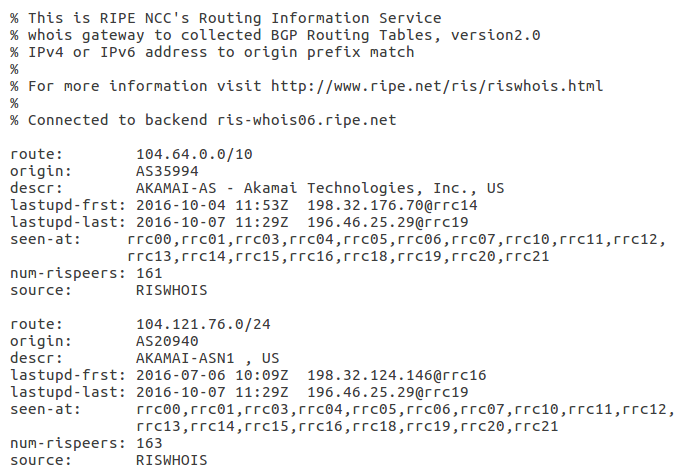
\includegraphics[width=\textwidth,height=10cm]{/home/sakib/soumya/latexNew/whois.png}
\centering
\caption{RIPE RIS bgp prefixes using whois command}
\end{figure}
From DNS resolution, the hosting infrastructure and corresponding IP addresses are determined. To find out BGP prefix routes of a particular IP address, BGP routing information from RIPE RIS [23] will be used. In figure-7, "route" shows the BGP prefixes of a IP address. From the figure this can be observed that the IP address 104.121.76.73 can be routed via two different prefixes 104.64.0.0/10 and 104.121.76.0/24. So both the prefixes for this IP will be considered for further analysis. This procedure will be carried out for each IP addresses of hosting infrastructure which will result in (hosting infrastructure, prefixes) mapping.

\subsection{Clustering}
From the initial analysis on the data collected for analyzing hosting infrastructure, it is found out that some hosting infrastructure are administered by the same company. For example, both the hosting infrastructure akamaiedge.net and akamai.net are administered by the same company, Akamai. Similarly google.com, googleusercontent.com, googlehosted.com and googledomains.com are administered by same company, Google. Generally companies use different ARecord names depending on the type of service they offer and the geographical location from where they offer the services. It is observed that Amazon uses two different ARecord names, namely amazonaws.us-east-1.elb.amazonaws.com, eu-west-1.elb.amazonaws.com for its customers from two geographical locations. It has to be analyzed, whether these ARecord names are pointing to same infrastructure or different. If they are pointing to the same infrastructure, they should be considered as one, else separately. This can be identified by using clustering algorithm by analyzing the BGP prefixes they share. 

The clustering algorithm takes a two step approach. In the first step, the prefixes of the hosting infrastructure will be aggregated into set of parent prefixes as explained in 3.2.1. In the subsequent step, the parent prefixes of the hosting infrastructure will be compared with each of the remaining infrastructure for clustering as explained in section 3.2.2.
\subsubsection{Prefix Aggregation of hosting infrastructure}
From the section 3.1.2, hosting infrastructure mapped to corresponding BGP prefixes are collected. But in this mapping, it is observed that some of the BGP prefixes are subset of other BGP prefixes. For example, googledomains.com has the prefix set ’216.239.32.0/19’, ’216.239.32.0/24’, ’216.239.34.0/24’, ’216.239.36.0/24’ and ’216.239.38.0/24’. Here the prefixes ’216.239.32.0/24’, ’216.239.34.0/24’, ’216.239.36.0/24’, ’216.239.38.0/24’ are subnet of prefix ’216.239.32.0/19’. Hence it is ideal to aggregate them. This way all the child prefixes in each mapping are aggregated to their parent prefixes. By end of this method, each hosting infrastructure will be mapped to a set of parent prefixes. For example, the hosting infrastructure googledomains.com is mapping to the parent prefix ’216.239.32.0/19’, as all child prefixes got aggregated into '216.239.32.0/19' parent prefix. This procedure is repeated for all the other infrastructure mappings, which generates a complete list of hosting infrastructure to their corresponding aggregated BGP prefixes.These mapping are sorted in the decreasing order of links hosting by each of these hosing infrastructure.The motivation behind doing this, is to allow the merging of smaller infrastructure into the larger one depending on their similarity factor (sim(s1, s2)) which is discussed in next section.

\subsubsection{Evaluation of Similarity between two hosting infrastructure}
The possibility of clustering any two hosting infrastructures is determined by analyzing the similarity between their aggregated prefixes. This can be done by verifying if one prefix is a parent to the other. While comparing two hosting infrastructures, if any of the hosting infrastructure contain child prefix of other, then the child prefix will be replaced with the parent prefix. This will make two prefix sets homogeneous, thus helping in evaluating the degree of the similarity between them. For comparing two hosting infrastructures, the similarity equation is defined as follows,

The similarity factor sim(s1,s2) is defined as follows,
\begin{equation}
sim(s1, s2)= \frac{|s1 \cap s2|}{|s2|}
\end{equation}

where s1,s2 are the bgp prefix sets.

If the similarity between two prefix sets are greater than equal to the 70\%, then both the hosting infrastructure will be clustered together making them a single clustered infrastructure. It is assumption that, s2 can be clustered with s2, provided 70\% of s2's prefixes are from that of s1's. This procedure will be repeated for all the hosting infrastructure. If two infrastructure has similarity factor greater than equal to 0.7, then the child hosting infrastructure will be merged into the parent hosting infrastructure and will be excluded from further comparisons. For example ’googleusercontent.com’ matched with ’google.com’ with similarity factor 1. This does not mean that both these hosting infrastructure has the same set of prefixes, but it means that, ’googleusercontent.com’ shares 100\% of its prefixes with ’google.com’. Once this is matched, ’googleusercontent.com’ will not be available for any further similarity matching with any other hosting infrastructures. It is assumed that a similarity index of grater than equal to 0.7 served as a good measure to determine the degree of similarity between two hosting infrastructure which can be considered as future work for extensive analysis.A sample example is explained as follows,

\begin{center}
\fbox{\begin{varwidth}{\dimexpr\textwidth-2\fboxsep-2\fboxrule\relax}

Let (hosting infrastructure,Prefix set)s are,
(SLD1,[10.0.0.1/24,12.0.0.0/16,192.168.3.0/24])
(SLD2,[192.168.0.0/16,10.0.0.0/16,12.0.0.0/24])
(SLD3,[3.0.0.0/8,12.0.0.0/24,192.168.3.8/24,5.0.0.0/16])
(SLD4,[4.0.0.0/24,6.0.0.0/24,10.0.0.0/16])
(SLD5,[6.0.0.1/16,10.0.0.0/8])

After the clustering procedure, SLD2 and SLD3 will clustered with SLD1 creating (SLD1,(SLD2,SLD3))mapping and SLD5 will be clustered with SLD4 to create (SLD4,SLD5) mapping.

\end{varwidth}}
\end{center}

\subsubsection{Evaluation of hyper giants}
Once the clustering procedure is performed, a list of parent hosting infrastructure to child hosting infrastructure are available for further analysis. To find out hyper giants presence, the features of each clustered hosting infrastructures will be analyzed. The features include number of links, number of IP addresses, number of BGP prefixes, number of AS numbers. To find out each of these features for a  clustered hosting infrastructure, corresponding child hosting infrastructures  will be considered. Hence total number of links for a clustered hosting infrastructure will be the sum of all the links served by all child hosting infrastructures. To find out number of BGP prefixes,the set of two prefix sets will be taken. This will result the unique BGP prefixes. Similarly to get the AS numbers, the set of two prefix sets will be taken.
\begin{center}
\fbox{\begin{varwidth}{\dimexpr\textwidth-2\fboxsep-2\fboxrule\relax}
Let,
p = numner of links served by SLD1
q = number of links served by SLD2
r = number of links served by SLD3

and mapping is, p -> (q,r) which means SLD2 and SLD3 are clustered with SLD1
	then number of links of clustered hosting infrastructure = p + q + r (Each link will be considered separate) 
	
x = numner of IP addresses served by SLD1
y = number of IP addresses served by SLD2
x = number of IP addresses served by SLD3

and mapping is, x -> (y,z) which means SLD2 and SLD3 are clustered with SLD1
	then number of links of clustered hosting infrastructure = set(x,y,z) (This will give the unique bgp prefixes)
		
Let,
i = numner of bgp prefixes served by SLD1
j = number of bgp prefixes served by SLD2
k = number of bgp prefixes served by SLD3

and mapping is, i->(j,k) which means SLD2 and SLD3 are clustered with SLD1
	then number of BGP prefixes of clustered hosting infrastructure = set(i,j,k) (This will give the unique bgp prefixes)
	
Let,
a = numner of ASs served by SLD1
b = number of ASs prefixes served by SLD2
c = number of ASs prefixes served by SLD3

and mapping is, a->(b,c) which means SLD2 and SLD3 are clustered with SLD1
	then number of ASNs of clustered hosting infrastructure = set(a,b,c) (This will give the unique ASNs)

\end{varwidth}}
\end{center}

The features of clustered hosting infrastructure will be analyzed further to find out the hyper giants.

To identify the hyper giants, the hosting infrastructures with unique behavior will be separated from the others. To perform this, two main features will be taken, number of links and number of IP addresses. k-means algorithm [26] will be performed on clustered hosting infrastructure to partition the clustered hosting infrastructure in up to k clusters .The cluster co-efficient value k is chosen as 10.Clusters whose features have high values will be clustered together. On the other hand, smaller infrastructures that use very few links and IP addresses are
not sufficiently different, and therefore, can be found in the same cluster.To identify the hyper giants, the clustered hosting infrastructure which clustered separately than the most of the other clustered hosting infrastructure will be considered.

\subsection{Web objects delivered from hyper giants to popular web sites}
To find out different web objects delivered from hyper giants to popular web sites, HTTP header information for all URLs corresponding to each clustered hosting infrastructure is analyzed. From header information, the content type of each object can be extracted. This information is useful to determine what type of web objects are served by each hyper giant.
\subsection{Conclusion}
This section discussed about the methods to identify the presence of hyper giants in today's Internet and to find out the inter dependency between hyper giants and popular websites. To execute both the methods,IP addresses, AS numbers, BGP prefixes are used as features for categorical analysis of clustered infrastructure. The section provided the procedures to find out each of the features for hosting infrastructures. At the end, HTTP header information is used to determine the type of web objects served by each hyper giant.
\newpage

\section{Implementation}
This section describes how the first prototype of an crawler was built. It explains the
choice of programming language as well as go into some details of the objects, the rough internal working and their interaction with each other. In the end, the usage of the program will be explained briefly.

\subsection{Choice of programming language}
Before going for implementation,it is important to know that the whole process involve two major parts.In the first part,we use a web crawler to collect popular website links as well as embedded links.And in second part we are going to analysis these crawled data to find out our result.Hence we need to choose a programming language which should be powerful in development as well as can be used for data analysis.So that any kind of dependency between two procedure can be handled easily.Again language should be free, open and usable by anyone who wishes to run this crawler implementation.Again the language should have good number of open libraries,big community who can help in necessary and should have a lot of documentation available in Internet .For this purpose we choose python as it fulfills all necessary requirement. For development we are going to use python and for data analysis we will use python,pyspark (Python version of spark).

\subsection{Development Tools}
For development,it is important to choose correct IDE which allows us to write code in less time with minimum effort.Along with this it helps in code completion, syntax highlighting, debugging and refactoring.For this purpose we have chosen "sublime editor" which is free and easy to write python code.

Now second most important aspect is to choose python web crawling tool which will suit our requirement and can be used in future.We will focus on programs that request web services from service providers and programs that scrape data from web sites. Web service applications will involve us in a new kind of programming called client-server programming; the programs we will look at will be client programs making requests from service on the Internet. Although the underlying foundation of a web-scraping program is also a client-server interaction, we will use some tools that hide the details of those interactions, and allow us to fetch web page content directly.For this we have couple of choices which are well known web crawling tools like urlib,beautiful soup,scrapy etc. But Python Scrapy is the best out there, Scrapy crawling is faster than any other platforms, since it uses asynchronous operations (on top of Twisted). Scrapy has better and faster support for parsing (x)html on top of libxml2. Scrapy is a mature framework with full unicode, redirection handling, gzipped responses, odd encodings, integrated HTTP cache etc.Again it is open source having a big community and documentation.

There are lot of different machine learning tools available but as we expect out data to be of some gigabytes,it is better to use that tool which can process data faster.Python and R are popular languages for data scientists due to the large number of modules or packages that are readily available to help them solve their data problems. But traditional uses of these tools are often limiting, as they process data on a single machine where the movement of data becomes time consuming, the analysis requires sampling (which often does not accurately represent the data), and moving from development to production environments requires extensive re-engineering. Spark provides a powerful, unified engine that is both fast (100x faster than Hadoop for large-scale data processing) and easy to use.Hence we are going to Pyspark for our initial data analysis and then we well do further analysis using python and RStudio.

Apart from above tools we use some other tools for the implementation.The following are the list of important softwares and tools used.

\begin{itemize}
  \item dnspython:it is a DNS toolkit for python.This is used in the code to get the A records of hosts.
  \item pygeoip :The libarary is used to get the ASN numbers associated with IP addresses.This library is based on Maxmind’s GeoIP C API.
  \item urlparse :this is used to convert a relative url to an absolute url.
  \item Public suffix List :This is the collection of all registered host names given by all internet users.The Public Suffix List is an initiative of Mozilla, but is maintained as a community resource.It is available for use in any software, but was originally created to meet the needs of browser manufacturers.In our code we use it to get second level domain from a host name.The "effective\_tld\_names\. dat" is the file which is free downloadable from their site.
  \item IPython :IPython notebook is used for pyspark code writing and execution.
  \item matplotlib :Python library used to for making different graphs used in this thesis.
  \item pygal :Pygal is also another python library which we used to make graphs.
\end{itemize}

\subsection{Design of Crawler Engine}
In this section,we will discuss the whole architecture behind the implementation.The design process involves two parts,first one is the architectural overview of crawler engine which takes 100,000 top ranked websites of Alexa as input,crawl the websites , return result file as output from the engine and second part is processing of result file using data processing engine which internally use "pyspark".Along with this,we will also discuss little bit about "Scrapy framework" which is main backbone behind the crawler engine.The input to crawler and result output file matrices also will be discussed on the below section.

\subsubsection{Crawler Engine}
In this section we will discuss the internal architecture behind the crawler engine.We will start with "Scrapy framework" [19] which is the main crawler engine work behind the whole crawler engine.Scrapy framework is based on spiders which are self-contained crawlers worked by set of given instructions.As it is one of the top ranked open source project,lots of  documentation can be found.The main objective of crawler engine is to take input data in the format of text file which contain the top 100,000 websites of Alexa.Then divide this master domain list into multiple sub domain lists with equal weighted websites and then process each sub domain list using separate crawler instances.Each crawler instance work independently and store all website information like HTTP header information,rank of website in Alexa etc. in result file. 
\subsubsection{Scrapy Framework}
Scrapy framework is one of top ranked open source project used for,a fast web crawling framework,used to crawl websites and extract structured data from their pages.It provide option for both focused and broad crawling.In case of focused crawler scrapy crawls a specific domain while in case of broad crawling a large (potentially unlimited) number of domains.Hence for our implementation ,we are going to use the broad crawling.As we can see from figure-7,the main components of the framework contain scrapy engine,scheduler,downloaders,spiders,item pipeline,downloader middlewares.

\begin{itemize}
\item Scrapy Engine :
The engine is responsible for controlling the data flow between all components of the system, and triggering events when certain actions occur. 

\item Scheduler :
The Scheduler receives requests from the engine and enqueues them for feeding them later (also to the engine) when the engine requests them.

\item Downloader :
The Downloader is responsible for fetching web pages and feeding them to the engine which, in turn, feeds them to the spiders.

\item Spiders :
Spiders use for to parse responses and extract items from them or additional URLs (requests) to follow.

\item Item Pipeline :
The Item Pipeline is responsible for processing the items once they have been extracted (or scraped) by the spiders. Typical tasks include cleansing, validation and persistence (like storing the item in a database). For more information see Item Pipeline.

\item Downloader middlewares :
Downloader middlewares are specific hooks that sit between the Engine and the Downloader and process requests when they pass from the Engine to the Downloader, and responses that pass from Downloader to the Engine.

\end{itemize}
\begin{figure}[h]
\includegraphics[width=\textwidth,height=10cm]{/home/sakib/soumya/latex/scrapy_architecture}
\centering
\caption{Scrapy Architecture}
\end{figure}

\subsubsection{Scrapy data types}
Scrapy uses some specific classes and strings which are used to crawl data.These are written in python and are open source.Scrapy also use twisted framework for multi threading.Some of the classes which we are going to use for implementation are as follows,

\begin{enumerate}
   \item Spider :Spiders are the classes used to crawl single or multiple domains using different methods like start\_requests(),parse().
   \begin{itemize}
     \item start\_requests() :This scrapy method is used to pass domains to parse method for further crawling process.
     \item parse() :he parse method is in charge of processing the response and returning scraped data and/or more URLs to follow. Other Requests callbacks have the same requirements as the Spider class.
   \end{itemize}
      \item Twisted Framework:Twisted supports an abstraction over raw threads — using a thread as a deferred source. Thus, a deferred is returned immediately, which will receive a value when the thread finishes. Callbacks can be attached which will run in the main thread, thus alleviating the need for complex locking solutions. A prime example of such usage, which comes from Twisted's support libraries, is using this model to call into databases. The database call itself happens on a foreign thread, but the analysis of the result happens in the main thread.
      \item Requests objects:Typically, Request objects are generated in the spiders and pass across the system until they reach the Downloader, which executes the request.A Request object represents an HTTP request, which is usually generated in the Spider and executed by the Downloader, and thus generating a Response.
	\item Response objects :Request object returns a Response object which travels back to the spider that issued the request.A Response object represents an HTTP response, which is usually downloaded (by the Downloader) and fed to the Spiders for processing.

\end{enumerate}
\subsection{Workflow}
The whole workflow is divided into two steps.In first step divided the whole list of 100,000 domains ranked by Alexa into multiple sub lists.Each sublist then will be sent as input to multiple instances of scrapy.In the second step scrapy engine crawls each website link from sub lists and store the results.We will discuss both the steps in following subsections.
 \subsubsection{PreCrawling Step}
In precrawling step,main focus is to create multiple instances of scrapy spider.As scrapy is a large memory greedy tool,after testing we decided to create 20 parallel threads which work independently shown in figure 8.Each instance will take separate input file which contain 5000 domains .So we need to divide the master domain list into sublists but we also need to divide it such a way that all the crawlers will complete their crawling in almost same time.Hence we choose to create the sublists with equal weight.Weight points to rank of the websites here.

\begin{figure}[h]
\includegraphics[width=\textwidth,height=10cm]{/home/sakib/soumya/latex/archi-1}
\centering
\caption{Pre Creawling Step}
\end{figure}

The master domain list contain the the website url and the rank of the websites.So after division the first sublist will contain the websites of 1st rank,21st rank,...99981st rank;second list will contain 2nd rank,22nd rank...99982nd rank websites and so forth for other instances.Hence each sublist will contain 5000 websites with equal division of website ranks. 

\subsubsection{Crawling Step}
In this step each crawler will take 5000 domains and parse one by one domain to the crawler engine.For each url we download the corresponding web page, extract the linked URLs, and check each url to see whether the extracted url is a fresh url which has not already been seen . With this architecture we are essentially carrying out a very large number of independent crawls of the white listed domains obtained from Alexa.Along with HTTP header information,the crawler engine also extract Arecord details ,ASN details.

\subsection{Conclusion}
In this section we talked about the softwares we are going to use to complete the whole implementation.We talked about the motivation behind choosing different languages,software tools to complete the implementation.Again we discussed about the web crawler as well internal architecture of crawler engine.In the next section we will talk about the approach to collect traces, i. e., active DNS measurements, in order to evaluate our methodology.
\newpage

\section{Measurement}
\section{Measurement\label{cha:chapter5}}
\noindent In order to identify the presence of hyper giants in today's Internet and to find out the degree of dependency on hyper giants to delivery Internet web content, the 100,000 top ranked websites of Alexa are crawled. To find out the hyper giants, the hosting infrastructures which are serving popular websites are observed. DNS resolution and HTTP header information also extracted to identify the features related to each website link. The features are number of links served by each hosting infrastructure, number of IP addresses, number of BGP prefixes for each IP address and number of AS numbers. These features are used to cluster the hosting infrastructure following the methodology discussed in chapter \ref{cha:chapter3}. This chapter explains the overview of traces which are collected after each step staring from web crawling to the last step, web object identification.\\
\subsection{Web Crawling}
\noindent To obtain a good coverage of the hosting infrastructure, the 100,000 top ranked websites from Alexa [26] are crawled. Alexa ranks websites based on Internet traffic-users of its tool bar for various web browsers like Google Chrome, Internet explorer, Firefox . Moreover, websites contain a lot of embedded links to images, videos, advertisements etc. which the browser of the user has to download from the various web servers. These embedded links can be from different hosting infrastructure. In our study, such embedded links has to be taken into account, as it might be served from servers other than those serving the home page. To give a better understanding, while crawling facebook.com, the home page is served from Facebook hosting infrastructure while the logo and some other meta data come from Akamai. DNS resolution and HTTP header analysis is carried out on each of these web links including their corresponding embedded links to extract IP addresses, ARecord name information. The scrapy crawler queries the HTTP Get method to local DNS resolver for all the website links and store the results in a trace file.\\\\

\noindent Three sample traces are given below,\\

\begin{lstlisting}[caption= DNS Reply for a host using dig command line tool, label=lst:trace]

[55017, 0, 200, 'text/html', 19719,
 'http://parsquran.com',
  'a','parsquran.com', '74.208.215.213', 8560]

[55017, 1, 200, 'text/html; charset=UTF-8', 0, 
'http://parsquran.com/site/sitemap.html', 
'a', 'parsquran.com', '74.208.215.213', 8560]

[21794, 0, 200, 'text/html', 2014, 
'http://gomap.az', 
'a', 'gomap.az','85.132.44.164', 29049]

\end{lstlisting}

\noindent Each trace contain 10 different features, as described below.\\
\begin{enumerate}
   \item index: index shows the rank of the website.
	\item depth\_level: 0 or 1.
			  0 shows that the website is the main page url and 1 shows the embedded links inside main page 
\item httpResponseStatus: the HTTP return status code.
\item MIMEcontentType: this is included to know the type of element inside the web page.
\item ContentLength: content length gives the idea about the size of the element. The content type only extracted for the home page link.
\item URL: this is the URL to be crawled by the scrapy engine.This URL can be main page URL or embedded links.Duplicate links are omitted for the same main page by using RFPDupeFilter.RFPDupeFilter is a scrapy class which is used to detect and filter duplicate requests [20].
\item tagType :this shows the HTML element type.
		for example if an element is embedded in a website like "<img class="desktop" title="" alt="" src="img/bg-cropped.jpg">",then the tagtype will be "img". 
\item ARecord=This contain all the aRecord names involved in a website while resolving to the ip address.
\begin{lstlisting}[caption= DNS Reply for a host using dig command line tool, label=lst:dig]

; <<>> DiG 9.10.3-P4-Ubuntu <<>> www.bmw.com
;; global options: +cmd
;; Got answer:
;; ->>HEADER<<- opcode: QUERY, status: NOERROR, id: 60134
;; flags: qr rd ra; QUERY: 1, ANSWER: 4, AUTHORITY: 0, ADDITIONAL: 1

;; OPT PSEUDOSECTION:
; EDNS: version: 0, flags:; udp: 512
;; QUESTION SECTION:
;www.bmw.com.			IN	A

;; ANSWER SECTION:
www.bmw.com.		3600	IN	CNAME	cn-www.bmw.com.edgesuite.net.
cn-www.bmw.com.edgesuite.net. 3600 IN	CNAME	a1586.b.akamai.net.
a1586.b.akamai.net.	20	IN	A	104.121.76.64
a1586.b.akamai.net.	20	IN	A	104.121.76.49

;; Query time: 22 msec
;; SERVER: 127.0.1.1#53(127.0.1.1)
;; WHEN: Fri Oct 14 09:46:54 CEST 2016
;; MSG SIZE  rcvd: 143
\end{lstlisting}


\noindent From the Listing \ref{lst:dig}, it can be observed that, a1586.b.akamai.net. is the ARecord name for the the website "www.bmw.com" which will be stored in trace will under ARecord column.\\
\item destIP :this column stores the corresponding resolved ip addresses of the website.For example,for the website bmw.com,the destIP will store 72.247.184.130 and 72.247.184.137
\item ASN\_Number=Field():This column stores the ASN number of a IP address.For this we use maxmind IP to ASN mapping file.
    \end{enumerate}
    
\noindent This procedure resulted in a total number of 12120731 unique links, which includes 100,000 top website links of Alexa, along with their embedded links.\\

\subsection{Data Cleanup}
\noindent From the traces that are collected in previous section, there might exist some traces for which one or more of the fields are missing, making them invalid. Such traces should be excluded from further analysis. This process of data cleaning are carried out by using regular expressions to filter out the invalid entries.\\

\subsection{Hosting infrastructure to BGP mapping}
\noindent As explained in section 3.1.1, the tests are carried to find out hosting infrastructure to corresponding BGP prefixes set. The IP addresses and corresponding BGP prefixes collected through RIPE RIS for hosting infrastructure, facebook.com is shown in table below.\\\

\begin{table}[htb]
\centering
\begin{tabular}[t]{|p{.3\textwidth}|p{.3\textwidth}||p{.3\textwidth}|}
\hline
SLD Infrastructure     & IP address&BGP Prefixes\\
\hline
\hline
facebook.com   & '173.252.88.112', '173.252.88.113', '173.252.88.104', '173.252.88.66', '173.252.90.132', '173.252.88.73'    &'173.252.88.0/21', '173.252.64.0/19'\\
\hline
\end{tabular}
\caption{Sample example shows SLD to BGP prefix mapping}
\label{tab:s1approcsupport}
\end{table}


\noindent From Table \ref{tab:s1approcsupport}, it can be observed that, the hosting infrastructure facebook.com in column-1 might have hosted several web links that are resolved to the above stated 8 IP addresses as stated in column-2 which can be reached through the set of prefixes as in column-3.\\

\subsection{Clustering}
\noindent There are some hosting infrastructure which are administered by same company. For example, both the hosting infrastructure akamaiedge.net and akamai.net are administered by the same company,Akamai. In such cases i tis verified whether these hosting infrastructure share common infrastructure, i which case are clustered together, following the clustering algorithm as described in section 3.2. This procedure is carried out for all the 219604 unique hosting infrastructure, which has resulted in 53852 unique clustered hosting infrastructure.\\

\noindent To find out hyper giants presence, the features of each clustered hosting infrastructures are analyzed. To find out the feature set of each clustered hosting infrastructure, the corresponding feature set of all the hosting elements involved is aggregate together as described in section 3.2\\

\noindent The  Table \ref{tab:s1approcsupport1} lists top 20 clustered hosting infrastructure on decreasing order of their number of links they host.\\\

\begin{table}[htb]
\centering
\begin{tabular}[t]{|p{.1\textwidth}|p{.4\textwidth}||p{.1\textwidth}||p{.1\textwidth}|p{.1\textwidth}||p{.1\textwidth}||p{.1\textwidth}|}
\hline
sl. no.& Clustered SLD Infrastructure    & SLDs & links& IP addresses& ASNs& prefixes \\
\hline
\hline
1&cloudflare.net& 17711& 1295505& 29893& 17 &78\\
2&akamaiedge.net& 158& 597533& 3396& 9 &27\\
3&google.com& 251& 240910& 195& 1&22\\
4&yunjiasu-cdn.net& 6068& 210463& 5907& 21&77\\
5&us-east-1.elb.amazonaws.com& 4254& 199109& 10885& 31&115\\
6&wpengine.com& 3963& 136400& 4072& 19&115\\
7&anycast.me& 2667& 116024& 2207& 3&13\\
8&ourwebpic.com& 722& 113746& 772& 16&16\\
9&eu-west-1.elb.amazonaws.com& 1946& 100265& 4476& 25&31\\
10&kxcdn.com& 1547& 82120& 1235& 7&7\\
11&edgecastcdn.net& 73& 79750& 383& 2&11\\
12&jiashule.com& 1769& 79038& 2249& 28&100\\
13&cloudflare.com& 3& 78907& 34& 1&5\\
14&alikunlun.com& 964& 76647& 1155& 17&45\\
15&d5nxst8fruw4z.cloudfront.net& 3331& 75660& 1619& 3&7\\
16&incapdns.net& 35& 66882& 382& 7&27\\
17&fastlylb.net& 73& 65360& 201& 0&4\\
18&dynect.net& 1& 62760& 46& 2&5\\
19&ap-northeast-1.elb.amazonaws.com& 1308& 60343& 3105& 22&23\\
20&d2t8dj4tr3q9od.cloudfront.net& 2363& 59807& 1316& 8&7\\
\hline
\end{tabular}
\caption{top 20 clustered hosting infrastructure}
\label{tab:s1approcsupport1}
\end{table}

\noindent The columns 1-6 from table represent name of the clustered hosting infrastructure, number of hosting infrastructure that are merged into the same cluster, number of links collectively hosted by the cluster, collective set of IP addresses of the cluster, collective number of ASNs of the cluster and collective  BGP prefixes of the cluster respectively.
From table, it can be observed that 17711 number of SLDs merged with cloudflare.net. From the table it can be observed that two different clustered hosting infrastructure in sl. no. 1, 13, belonging to the same company, cloudflare but remained in different clusters.This is because, they have different infrastructure from each other in terms of BGP prefixes. Same is the case for hosting infrastructure in sl. no. x,y,z administered by Amazon. This might be because of big hosting infrastructure use different infrastructure for various operations.\\

\subsection{Candidate Analysis for hyper giant}

\begin{figure}[htb]
  \centering
  \includegraphics[width=14cm]{/home/sakib/soumya/wholeSLD/graphs/clubbedSLDWhole.png}\\
  \caption{Number of SLDs served by different SLD infrastructure clusters}
  \label{fig:SLD}
\end{figure}

\noindent From Figure \ref{fig:SLD} it can be seen that, almost 80\% of the total unclustered hosting infrastructure got clustered into first 3.73\% of hosting infrastructure. Many of the other hosting infrastructure share their infrastructures with these top 3.73\% of clustered infrastructures. Hence there is a possibility to get the hyper giants in these 3.73\% of clustered hosting infrastructure. But there are hosting infrastructure who have their own infrastructure in the form of data centers. Hence they don't share any other hosting infrastructure. Like facebook.com who has its own infrastructure in the form of data centers all over the world. In fact from figure ,it is also observed that almost 82.45\% of clustered infrastructure who does not share their infrastructure with no more than another hosting infrastructure. It means there are companies who work independently by creating their own infrastructure.This can be data centers all over world. Although these 82.45\% of clustered infrastructure do not share their infrastructure with no more than single infrastructure, still some of them serve a large number of links which make them another candidate for hyper giant analysis.\\

\noindent Hence to get a better picture, the clustered hosting infrastructure will be analyzed based on how many links they served. Hence by sorting all clustered hosting infrastructure in their decreasing order of links, it is found that top 5.95 \% (=3205) clustered hosting infrastructure serve almost 80\% of links and have 78.65 \% of hosting infrastructure. Hence hyper giants can be found in this range.\\

\subsection{Collection of web objects}
\noindent Different web objects embedded in home pages of 100,000 top ranked web sites of Alexa are also collected.After crawling, it is observed that total 285 different types of objects from 13919464 links present in Internet. 38\% of all the URLs constitute of object type text, while 42 \% of URLs constitute of object type image.\\

\subsection{Conclusion}
\noindent This chapter outline the measurements obtained after crawling the 100,000 top ranked websites of Alexa. This has resulted in total of 13919464 links which include both the home pages of these top ranked websites and their corresponding embedded links. After applying DNS resolution on these links, 219604 hosting infrastructure are detected. On clustering these infrastructure, it has resulted in total 53852 clustered hosting infrastructure. It is found that the top 5.95\% clustered infrastructure alone are serving 80\% of all URLs. It is also found out that 78.65 \% of hosting infrastructure pools into the same 5.95\% clustered infrastructure. It is for this reason, it can be conveniently assumed that the hyper giants are exists in these top 5.95 \% of clustered hosting infrastructure, owing to zipf's law. The measurements revealed that all the URLs constitute 38\% of object type text/html, while 42 \% of URLs are of the object type image.\\

\newpage

\section{Results}
This chapter analyzes the measurements obtained from chapter 5 to identify hyper giants by studying the features of clustered hosting infrastructure such as number of links served by the cluster, number of IP addresses that belong to the cluster, number of BGP prefixes to reach the cluster, number of AS numbers that belong to cluster. Once hyper giants are determined, the dependency of popular websites on them will be examined by taking into consideration that the type of web objects like images, videos, HTML files etc delivered by these hyper giants. 

\subsubsection{Identifying hyper giants}

\subsubsection{case 1 :number of Links Vs number of IP addresses}
In this section we will take the top 3205 SLD infrastructures and cluster them based on their number of links to ip addresses they served.

\begin{figure}[h]
\includegraphics[width=\textwidth,height=10cm]{/home/sakib/soumya/wholeSLD/Rplot.png}
\centering
\caption{Clustering based on links and IP address features}
\end{figure}

We used k-means clustering algorithm and number of cluster parameter 10.We found 6 different clusters which are clubbed total 26 SLD infrastructures and showing unique behavior.Like cloudflare.net is clustered separately as it is serving very huge number of links as well as having very high number of ip addresses.It means lots of small SLDs are serving through cloudflare.net and it has footprint all over the world.Similarly us-east-1.elb.amazonaws.com clustered separately as it has less high of links but serving a high number of ip addresses.third cluster contain google.com which is serving high number of links but not very high number of ip addresses.In this way we are able to identify total 6 clusters which resulted in a total of 26 SLD infrastructures. But it is difficult to categorize them into some specific type of infrastructure based on only  links to ip address analysis. Hence these 26 SLD infrastructures will be further analyses taking into account their prefixes to their asn numbers.

\subsubsection{case 2 :number of BGP Prefixes Vs number of ASNs}
From last section we identify the SLD infrastructures which are having unique behavior. But we couldn't able to classify them .Therefore in this step we will check how they are distributed all other world.This requires these clusters to be analyzed using their corresponding ASN to prefix numbers.This is because number of ip prefixes shows the footprint of the infrastructures across the world and the number of asn numbers show the degree of distribution of infrastructures across the world.
\begin{figure}[h]
\includegraphics[width=\textwidth,height=10cm]{/home/sakib/soumya/wholeSLD/prefixVsasn.png}
\centering
\caption{Classification of hyper giants}
\end{figure}

From figure-14 ,we can cluster all the clustered SLD infrastructures into 5 parts based on their <number of prefixes,number of ASNs> analysis as below.

\begin{itemize}
\item very high,very high :
In total 3 different clustered SLD infrastructures are clustered under this.
They are yunjiasu-cdn.net,jiashule.com,
us-east-1.elb.amazonaws.com.These three SLD infrastructures contain very high number of prefixes as well as they have high number of ASN numbers,which shows that they have footprint all over the world  as well as they are distributed across the world.We can classify them as highly distributed CDNs.
\item high,high : 
Total 7 SLD infrastructures clubbed inside this. wpengine.com
,alikunlun.com,cloudflare.net,ourwebpic.com,
us-west-2.elb.amazonaws.com,eu-west-1.elb.amazonaws.com and 
ap-northeast-1.elb.amazonaws.com.They have high number of footprint and high number of asn numbers.This shows they have presence in few of the regions.We can classify them as distributed CDNs.
\item high,less  :
netdns-cdn.com and cdntip.com
These SLD infrastructures have high number of prefixes but have less number of ASN numbers.It means they have footprint all over the region but they normally administered through very few ASN numbers.Hence these can be categorized into cloud computing infrastructures. 
\item  medium,medium :
Five different SLD infrastructures are clubbed into same cluster.They are,
akamaiedge.net,ap-southeast-1.elb.amazonaws.com,
kxcdn.com,incapdns.net,d2t8dj4tr3q9od.cloudfront.net
 All these infrastructures have few prefixes and they also not distributed which gives an evidence of multi homes data centers or web hosting companies.
\item less,less :
The rest of the CDN infrastructures are clubbed into same cluster which having very few number of prefixes also very few number of IP addresses.Hence they can be treated as content providers.Google and Microsoft both clustered under this.
\end{itemize}

\pagebreak
\subsubsection{Conclusion}
From the above section,we are able to identify total 26 hyper giants which are having influence in Europe region.They are highly distributed CDNs,cloud platforms,CDNs,content producers etc.In next section we will see how they influence on number of objects delivered by them.

\subsection{Popular websites dependency on hyper giants}
In this section,first we will see different types of objects delivered through 219604 unique SLDs and compare this with web objects delivered by 26 hyper giants. Then we will examine each hyper giant separately and try to find what kind of data object they deliver. 
\subsubsection{Object types delivery through whole SLD infrastructures Vs hyper giants}
\begin{figure}[h]
\includegraphics[width=\textwidth,height=10cm]{/home/sakib/soumya/wholeSLD/objectCount.png}
\centering
\caption{top 10 object percentage used by all SLDs}
\end{figure}
\begin{figure}[h]
\includegraphics[width=\textwidth,height=10cm]{/home/sakib/soumya/wholeSLD/objectCount/hypergiant.png}
\centering
\caption{top 10 object percentage used by all hyper giants}
\end{figure}

Figure-15 and figure-16 shows top 10 object types in terms of their percentage of the total web objects they served .In case of hyper giants top 10 object types deliver almost 98.82 \% of the total object types they host. It can be inferred from the graph that hyper giants host 68.27\% of HTML object type making it the single highest contributor to the total web objects it hosts. 


Furthermore, 75.04\% of the total object types it hosts are of text object type such as text/html,text/css,text/xml,text/js etc. Furthermore, 18\% of the total object types it hosts are of image object type such as image/png and image/jpeg. 

, are delivered through hyper giants where as only 19.29\% of image files delivered through hyper giants.



In case of SLDs,top 10 object types carries almost 97.94\% of all object types  which is very much similar to the percentage of objects delivered by hyper giants.The highest web object type delivered through all SLDs as well as hyper giants is text/html but it can be observed that in case of all SLDs,text/html carries almost 38\% of all web objects which is around 68.27\% in case of delivering through hyper giants.In case of all SLDs ,object types are distributed properly.If we add image/jpeg,image/png,image/gif then all SLDs serve more image files than HTML files.But same is not the case for hyper giants.Similarly it can be seen that almost 46.77\% of text files delivered through whole sld set which is almost 1.5 times more in case of hyper giants.But in case of image files ,SLDs serve almost 42 \% of all web objects which is almost double the image files served through hyper giants.This different behavior might be because popular content websites normally store more dynamic files in CDNs where as in case of image files they store at their own servers.

\subsubsection{Object types delivered from hyper giants to popular web sites}
In this section we will see what kind of data mostly delivered through the identified hyper giants.In today's Internet ,content plays most vital role.Hence it is important to observe what kind of data mostly delivered through hyper giants .
\newline
\newline
\begin{tabular}{ |p{6cm}||p{2cm}|p{2cm}|p{2cm}| }
 \hline
 \multicolumn{4}{|c|}{Hyper giant Object List} \\
 \hline
 Country Name     & text&image&application\\
 \hline
 alikunlun.com   & 75.99    &20.32&   3.65 \\
d2t8dj4tr3q9od.cloudfront.net&   49.86  & 41.10   &8.68\\
 ap-northeast-1.elb.amazonaws.com &90.28 & 6.23&  3.44\\
 ap-southeast-1.elb.amazonaws.com    &87.94 & 7.36&  4.62\\
 cdntip.com&   87.94  & 7.36&1.67\\
 d5nxst8fruw4z.cloudfront.net& 31.90  & 57.42   &10.23\\
 eu-west-1.elb.amazonaws.com& 87.25  & 7.32&5.39\\
 fastlylb& 69.79  &21.30&8.69\\
 google.com&82.54  & 15.79&1.65\\
 jiashule.com& 88.85  & 8.33&2.80\\
 kxcdn.com& 75.62  & 17.98&6.34\\
pbwstatic.com& 83.18  &16.57&0.24\\ 
 akamaiedge.net&73.65  & 20.35&5.93\\ 
 anycast.me& 79.64  & 14.90&5.37\\
 cloudflare.net& 64.86  & 11.98&23.12\\
 cloudflare.com& 78.15  & 15.62&1.70\\ 
dynect.net& 94.53  & 3.74&3.74\\
 edgecastcdn.net& 53.23 & 38.44&8.17\\ 
incapdns.net& 64.86  & 7.61&4.81\\
 netdna-cdn.com& 21.08  & 55.04&23.39\\ 
ourwebpic.com& 86.56  & 11.58&1.84\\
 us-east-1.elb.amazonaws.com& 88.99  & 6.18&4.73\\ 
wpengine.com& 80.67  & 12.42&6.84\\
 us-west-2.elb.amazonaws.com&85.30  & 8.15&6.47\\ 
windows.net& 80.52  & 12.99&6.41\\
 yunjiasu-cdn.net& 87.76  & 9.86&0.0\\ 
 \hline
\end{tabular}
\newline

The table shows all 26 hyper giants and the percentage of text,image and application web objects delivered by them.We can see from table than most of the hyper giants deliver very high percentage of text files which contain text/html,text/css etc.But their are few exceptions .Like both the cloudfront SLDs are providing very high number of images compare to other hyper giants.  Similar kind of observation can be seen for netdna-cdn which provides more image files than text files.

From last section we observed yunjiasu-cdn.net,jiashule.com, us-east-1.elb.amazonaws.com
 are highly distributed CDNs.It can be observed that all the three CDNs are delivering very high number of text files compare to image and application files.This might be because of their footprint all over the world and also have massively distributed CDNs.Hence they cache more of the HTML  files at edge servers to provide better performance.Similarly observation can be seen from  distributed CDNs .These CDNs also deliver high number of HTML files compare to image files but as they have presence in some regions the number of HTML files are not that comparable to highly distributed CDNs.Third infrastructure type we observed was cloud computing infrastructures and netdns-cdn.com,cdntip.com clustered under that.From the table it can seen that  netdns-cdn.com delivers more images and very less number of HTML files.Again cdntip delivers highest number of application data.The data centers provide both images and HTML files in a  very balance way.cloud front delivers 49\% of HTML file and 41\% of image files.Similarly akamaiedge.net provide around 20\%  of images.Content providers like window.net and google.com delivers very high number of links compare to number of images.This is evident as they have more content . 

\subsubsection{Conclusion}
From the section we can infer that both SLDs and hyper giants deliver maximum number of text/HTML files but it also found that hyper giants delivered almost 1.5 times more HTML files than SLDs.Same kind of observation can be seen for image files where SLDs deliver double the image content than hyper giants.Again we found that highly distributed CDN generally deliver more HTML links compare to image or application files which might be because of their massive CDN distribution.Distributed CDNs provide high number of HTML files because of their  presence in few regions.Cloud computing cdns provide more images than HTML file which might be because cloud computing provide scalability.Data centers delivers both HTML file and images in almost same ratio.Content providers also delivers more HTML files compare to image files which because of their rich content.

\newpage

\section{Conclusion}
\section{Conclusion\label{cha:chapter7}}
\noindent This thesis conducted an empirical analysis to find out the presence of hyper giants on Germany's Internet ecosystem. It aims to answer the following research questions: Firstly, whether there is any presence of hyper giants in today's Internet? Secondly, what web objects contained in popular websites are delivered through hyper giants? \\

\noindent To answer the first question, we introduced an automated process to find out the hosting infrastructure in today's Internet as well as cluster these hosting infrastructure to find out the presence of hyper giants. To perform this task, 100,000 top ranked websites of Alexa are crawled using scrapy engine and their HTML codes are inspected to retrieve all their embedded URLs. Using DNS resolution and HTTP header analysis, different features of hosting infrastructure are collected such as number of links, number of IP addresses, number of BGP prefixes, number of ASNs. A clustering algorithm is presented which will help to find out which hosting infrastructure are sharing infrastructure with each other using features of hosting infrastructure. The advantage of this automated approach is that, it uses SLD and BGP prefixes to perform the tasks, hence this procedure can be used in any other research. The study reveals that there are 26 hyper giants present in Internet when analyzed from a single vantage point in Germany, which are collectively contributing to nearly 30\% percentage of total web traffic on Internet. Some well known hosting infrastructure are detected in these 26 hyper giants, such as Google, Akamai, Amazon, Cloudflare etc.\\

\noindent The thesis has also focused on finding out, what web objects contained in popular websites are delivered through hyper giants. Using HTTP header analysis, different web object types such as text/html, image, video, audio etc. are collected. It is found that majority of the hyper giants focuses on delivering more number of text/HTML object files than other object types. This reveals that any disruption on hyper giant infrastructure may leave many web pages being unloaded. It is found that cloudflare.net delivered maximum percentage of \enquote{application} type web objects compared to other type of objects that it hosts. Google, Akamai are hosting more text/html object type files compared to other object types. cloudfront.com and netdna-cdn.com are delivering more image files compare to other web object types they host. This information will help the websites, which are focused on delivering a particular kind of content. For example video sharing sites are mainly focused on video content where as blogs focus more on text/html objects.This information might be of some value for this kind of web sites while they are making a decision on where to host their content. \\

\noindent The data is collected at a single vantage point in Germany. Furthermore this thesis is an important step towards answering some of the very crucial questions for CDNs, content providers etc. Moreover it will help the research community to discover the Internet architecture changes with time. They also can able to track the hyper giants and dependency of popular websites in these hyper giants.\\

The following areas can be investigated further which are not covered in the current scope of this thesis.

\begin{itemize}
\item Measurements are performed on a single vantage point in Germany. Hence the identification of hyper giants, their role and the degree of dependency of popular websites on hyper giants might change when the whole procedure will be carried out from multiple vantage points across the world. 

\item Secondly while clustering the hyper giants,the k-means parameter is taken by going through very small number of observations.Hence in future this can be tested more precisely which might help to cluster the hosting infrastructures at a granular level.

\item In the clustering algorithm, a similarity index of 0.7 is chosen to decide that two infrastructure can be clustered together. While this is an assumption, further analysis can be done on choosing the right similarity index.

\end{itemize}

\newpage

\section{Future Work}
There are certain areas which can be investigated further in future which are not covered in the current scope of this thesis.This section will discuss about these points.

\begin{itemize}
\item First of all the thesis is done at single vantage point at Germany.Hence the identification of hyper giants,their role and their relationship with popular websites can be changed when the whole procedure will be done in whole world basis.Hence it will be interesting to see how the clustering algorithm works when taking all the SLDs across the world.

\item Secondly while clustering the hyper giants,the k-means parameter is taken by going through very small number of observations.Hence in future this can be tested more precisely which will help to cluster the hosting infrastructures at a granular level.

\item In the clustering algorithm,we club two SLDs if one SLD prefixes matches with other SLD prefixes by more than equal to 70\%.This matching index is chosen after extensively testing.Hence this can be taken as future work to see what is the best matching index.

\item After clustering algorithm,we have chosen to take  top 5.95 \% (=3205) clustered SLD infrastructures which serve almost 80\% of links and have 78.65 \% of SLDs .In this way we argumented to get most of the big hosting infrastructures as well as content providers for further analysis.Hence this can be taken for future work to validate the argument properly.

\end{itemize}
\newpage

\section{Appendix}
\section{Cluster SLD infrastructure} 
Three different Clustered SLD infrastructure and corresponding SLD infrastructures are shown in table,

\begin{tabular}{ |p{3cm}||p{9cm}| }
 \hline
 \multicolumn{2}{|c|}{Clustering} \\
 \hline
 Clustered SLD Infrastructure     & SLD infrastructures\\
 \hline
 'twitter.com' & 'digits.com', 't.co'\\
'google.com'& 'googledomains.com', 'chromium.org', 'brokeroficial.com', 'google.ps', 'google.pt', 'teraxhif.com', 'google.hn', 'google.com.do', 'google.al', 'crossmediapanel.com', 'spellup.withgoogle.com', 'google.co.zw', 'shpargalkablog.ru', '1e100.net', 'google.hr', 'google.com.bz', 'google.pl', 'google.hu', 'google.co.ma', 'mrdoob.com', 'aminhaalegrecasinha.com', 'gosarkarinaukri.co.in', 'google.com.ly', 'google.com.bd', 'richmediagallery.com', 'lovefortechnology.net', 'golang.org', 'zagat.com', 'google.co.mz', 'google.com.lb', 'google.com.ag', 'google.com.gh', 'google.com.gi', 'rootupdate.com', 'google.am', 'google.com.cu', 'google.co.za', 'google.bs', 'google.co.zm', 'google.is', 'google.co.bw', 'fashionablygeek.com', 'google.co.ke', 'google.it', '2ality.com', 'osvelhotesdosmarretas.com', 'google.iq', 'google.jo', 'google.ae', 'google.ad', 'gametop.com', 'soberlook.com', 'gundam-vs.jp', 'google.ie', 'google.bj', 'google.co.jp', 'atomlabor.de', 'animesan1.com', 'google.com.vc', 'google.at', 'google.as', 'joancoscubiela.cat', 'google.no', 'google.nl', 'miroivanov.com', 'events.withgoogle.com', 'thisisyouramigaspeaking.com', 'google.ng', 'nanox-cp.jp', 'mediacrooks.com', 'schema.org', 'echridz.com', 'google.com.jm', 'google.co.tz', 'doubleclick.net', 'google.com.br', 'google.com.uy ,......\\
 'awsdns-40.com' &  'awsdns-16.com', 'srv1-trovit.ma', 'awsdns-33.com', 'awsdns-49.com', 'awsdns-22.com', 'awsdns-50.com', 'awsdns-21.com', 'awsdns-36.com', 'awsdns-52.com', 'awsdns-29.com', 'awsdns-06.com', 'awsdns-23.com', 'awsdns-12.com', 'awsdns-39.com', 'awsdns-31.com', 'awsdns-47.com', 'awsdns-43.com', 'awsdns-15.com', 'awsdns-02.com', 'awsdns-41.com', 'awsdns-00.com', 'awsdns-51.com'\\
\hline
\end{tabular}
\newline
\newpage

\section{List of Acronyms}
\begin{tabbing}
spacespacespace \= space \kill
CDN 	 \> Content delivery network \\
SLD 	 \> Second level domain \\
ASN	 \> 	Autonomous system number	 \\
BGP 	 \> Border gateway protocol \\
HTTP  \> Hypertext transfer protocol	 \\
HTML  \> Hypertext markup language	 \\
DNS  \> Domain name system	 \\
IP	 \> 	Internet protocol	 \\
QoS	 \> 	Quality of service	 \\
XML	 \> 	Extensible markup language	 \\
ISP	 \> 	Internet service provider	 \\
CDI	 \> 	Content delivery infrastructure	 \\
IaaS	 \> 	Infrastructure as a service	 \\
PaaS	 \> 	Platform as a service	 \\
SaaS	 \> 	Software as a service	 \\
IXP	 \> 	Internet exchange point	 \\
GGC	 \> 	Google global cache	 \\
CNAME	 \> 	Canonical name	 \\
RR	 \> 	Resource record	 \\
URIs	 \> 	Uniform resource identifiers	 \\
URL	 \> 	Universal resource locator	 \\
IDE	 \> 	Integrated development environment	 \\

\end{tabbing}


\newpage

\begin{thebibliography}{}
\bibitem{bib1}
\textit{http://www.internetsociety.org/globalinternetreport/assets/download/IS_web.pdf}
\bibitem{Leighton}
T. Leighton
\textit{Improving Performance on the Internet}.
Commun. ACM, 52(2):4451, 2009.
\bibitem{Labovitz}
C. Labovitz, S. Lekel-Johnson, D. McPherson, J. Oberheide, and F. Jahanian. 
\textit{Internet Inter-Domain Traffic}.
In Proc. ACM SIGCOMM, 2010.
\bibitem{Poese}
I. Poese, B. Frank, B. Ager, G. Smaragdakis, and A. Feldmann.
\textit{Improving Content Delivery using Provider-Aided Distance. Information}. 
In ACM IMC, 2010.
\bibitem{Maier}
G. Maier, A. Feldmann, V. Paxson, and M. Allman.
\textit{On Dominant Characteristics of Residential Broadband Internet Traffic}.
In Proc. ACM IMC,2009.
\bibitem{Nygren}
Nygren, R. K. Sitaraman, and J. Sun. 
\textit{The Akamai Network:A Platform for High-performance Internet Applications}.
Syst. Rev., 44:219, August 2010.
\bibitem{Krishnan}
R. Krishnan, H. Madhyastha, S. Srinivasan, S. Jain,A. Krishnamurthy, T.
Anderson, and J. Gao. 
\textit{Moving Beyond End-to-end Path Information to Optimize CDN Performance}.
\bibitem{Krishnan1}
Internet evolution
\textit{https://atos.net/content/dam/global/ascent-whitepapers/ascent-whitepaper-internet-evolution.pdf}
\bibitem{Schonfeld}
Schonfeld, E. Eric Schmidts 
\textit{Gang Of Four:Google, Apple,Amazon,And Facebook}.
TechCrunch.Retrieved from https://techcrunch.com/2011/05/31/schmidt-gang-four-google-apple-amazon-facebook/
\bibitem{Bernhard}
Bernhard Ager,Wolfgang Mhlbauer,Georgios Smaragdakis,Steve Uhlig
\textit{Web Content Cartography.}
\bibitem{Ager}
Bernhard Ager 
\textit{Impact of Location on Content Delivery}.
http://people.ee.ethz.ch/~bager/papers/A-ILCD-11.pdf
\bibitem{Yuval}
Yuval Shavitt, Udi Weinsberg.
\textit{Topological Trends of Internet Content Providers}.
SIMPLEX 12: Proceedings of the Fourth Annual Workshop on
Simplifying Complex Networks for Practitioners (2012): 13-18.
\bibitem{Xenofontas}
Xenofontas Dimitropoulos, Dmitri Krioukov, Marina Fomenkov, Bradley
Huffaker, Young Hyun, kc claffy, George Riley 
\textit{AS Relationships: Inference and Validation}.
SIGCOMM Computer Communications Review 37, no. 1(2007): 31-40.
\bibitem{Manuel}
Manuel Palacin, Miquel Oliver, Jorge Infante, Simon Oechsner and Alex
Bikfalvi 
\textit{The Impact of Content Delivery Networks on the Internet Ecosystem}.
Journal of Information Policy, Vol. 3 (2013), pp. 304-330
\bibitem{Gerber}
A. Gerber and R. Doverspike.
\textit{Traffic Types and Growth in Backbone Networks}.
OFC/NFOEC, 2011.
\bibitem{Mike}
Mike Axelrod
\textit{The Value of Content Distribution Networks and Google Global Cache}.
\bibitem{Frank}
Benjamin Frank, Ingmar Poese, Georgios Smaragdakis,
Anja Feldmann, Bruce M. Maggs, Steve Uhlig,
Vinay Aggarwal, Fabian Schneider
\textit{Collaboration Opportunities for
Content Delivery and Network Infrastructures}.
2013
\bibitem{Netflix Open Connect}
Netflix Open Connect
\textit{https://openconnect.netflix.com/en/}
\bibitem{Mike1}
\textit{http://www.hpl.hp.com/research/idl/papers/ranking/adamicglottometrics.pdf.}
\bibitem{Mike2}
Scrapy
\textit{http://doc.scrapy.org}.
\bibitem{Mike3}
\textit{Technology: How and Why We Crawl the Web}. 
Alexa. Archived from the original on April 2, 2014. Retrieved November 6, 2011.
\bibitem{Mike4}
P. Mockapetris
\textit{Domain Name System}.
https://www.ietf.org/rfc/rfc1034.txt
\bibitem{RISTOL}
K RISTOL , D., AND M ONTULLI , L. 
\textit{HTTP State Management Mechanism}.
RFC 2109.
\bibitem{RISTOL1}
K RISTOL , D., AND M ONTULLI , L.
\textit{HTTP State Management Mechanism}.
RFC 2965.
\bibitem{Lada}
Lada A. Adamic ,Bernardo A. 
\textit{Huberman Zipfs law and the Internet} . 
Glottometrics 3, 2002,p 143-150
\bibitem{Lada1}
RIPE NCC
\textit{RIPE Routing Information Service}.
http://www.ripe.net/ris/.
\bibitem{alexa}
Alexa
\textit{http://www.alexa.com/topsites}
\end{thebibliography}

\newpage

\newpage
\mbox{}
\cleardoublepage
\end{document}